
\subsection{Number Formatting Options}
\label{sec:number:printing}%
\PGFPlots\ typesets tick labels rounded to given precision and in configurable number formats. The command to do so is |\pgfmathprintnumber|; it uses the current set of number formatting options. In addition, \PGFPlots\ might prepare tick numbers before they are handed over to |\pgfmathprintnumber|.

The options related to number printing as such are described in all detail in the manual for \PGFPlotstable, which comes with \PGFPlots. This section contains the reference for everything which is specific to an axis, and only a brief survey over the number formatting options as such.

\subsubsection{Frequently Used Number Printing Settings}
\label{sec:number:faq}
This section provides a brief survey about the most frequently used aspects of number formatting in \PGFPlots. 
\begin{enumerate}
	\item \PGFPlots\ computes common tick scaling factors like $\cdot 10^2$ and produces only integers as tick labels.
	
	In order to get numbers like $0.001$ as tick labels instead of $1$ with a separate label $\cdot 10^{-3}$, you can use |scaled ticks=false| in your axis. See the description of |scaled ticks| for details.

	\item In order to customize the way numbers are rounded and/or displayed,
	use something like |xticklabel style={/pgf/number format/.cd,fixed,precision=5}|. 
	
	Here is a short list of possibilities:
\begin{codeexample}[]
\pgfmathprintnumber{123.456789}
\end{codeexample}
\begin{codeexample}[]
\pgfmathprintnumber{12345.6789}
\end{codeexample}

\begin{codeexample}[]
\pgfmathprintnumber
	[fixed,precision=5]{12345.6789}
\end{codeexample}

\begin{codeexample}[]
\pgfmathprintnumber
	[fixed,fixed zerofill,precision=5]{12345.6789}
\end{codeexample}

\begin{codeexample}[]
\pgfmathprintnumber
	[fixed,fixed zerofill,precision=5,use comma]
	{12345.6789}
\end{codeexample}

\begin{codeexample}[]
\pgfmathprintnumber
	[sci]{12345.6789}
\end{codeexample}

\begin{codeexample}[]
\pgfmathprintnumber
	[sci,sci zerofill,precision=5]{12345.6789}
\end{codeexample}

\begin{codeexample}[]
\pgfmathprintnumber
	[sci,sci generic=
	  {mantissa sep=\times,exponent={10^{#1}}}]
	{12.345}
\end{codeexample}

\begin{codeexample}[]
\pgfmathprintnumber[frac]{0.333333333333333}; 
	\pgfmathprintnumber[frac]{0.5}
\end{codeexample}

\begin{codeexample}[]
\pgfmathprintnumber[print sign]{2}
\end{codeexample}

\begin{codeexample}[]
\pgfmathprintnumber
	[1000 sep={\,},fixed,precision=6]{1000000.123456}
\end{codeexample}

\begin{codeexample}[]
\pgfmathprintnumber[
  1000 sep={\,},fixed,precision=6,
  1000 sep in fractionals]
	 {1000000.123456}
\end{codeexample}

	\noindent Each of these keys requires the prefix `|/pgf/number format/|' when used inside of a \PGFPlots\ style (try |/pgf/number format/.cd,|\meta{number formatting keys} to use the same prefix for many \meta{number formatting keys}).

	The number formatting uses |\pgfmathprintnumber|, a \pgfname\ command to typeset numbers. A full reference of all supported options is shipped with \PGFPlots: it is documented in the reference manual for \PGFPlotstable, Section `Number Formatting Options'. The same reference can be found in the documentation for \pgfname.

	Note that the number printer knows \emph{nothing} about \PGFPlots. In particular, it is not responsible for logs and their representation.

	\item For a logarithmic axis, one may want to modify the number formatting style for the \emph{exponent only}. In this case, redefine the style |log plot exponent style| (its documentation contains a couple of examples).

	\item In order to get |fixed| point tick labels on a logarithmic axis, you can use |log ticks with fixed point| (see below).
\end{enumerate}


\subsubsection{PGFPlots-specific Number Formatting}
This section contains fine--tuning options to change number formatting aspects -- but only things which are specific to \PGFPlots\ like peculiarities of tick labels on logarithmic axes. Consider browsing Section~\ref{sec:number:faq} first to see if you need this section. 

\begin{command}{\pgfmathprintnumber\marg{x}}
Generates pretty-printed output for the (real) number \meta{x}. The input number \meta{x} is parsed using |\pgfmathfloatparsenumber| which allows arbitrary precision.

Numbers are typeset in math mode using the current set of number printing options, see below. Optional arguments can also be provided using |\pgfmathprintnumber[|\meta{options}|]|\marg{x}.

Please refer to the manual of \PGFPlotstable\ (shipped with this package) for details about options related to number-printing.
\end{command}

\begin{stylekey}{/pgfplots/log ticks with fixed point}
	Reconfigures \PGFPlots\ to display tick labels of logarithmic axes using \emph{fixed point} numbers instead of the exponential style.

\begin{codeexample}[]
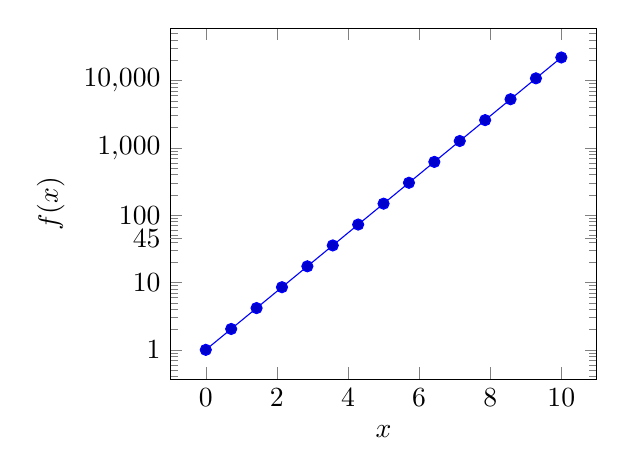
\begin{tikzpicture}
\begin{semilogyaxis}[log ticks with fixed point]
	\addplot+[domain=0:10] {exp(x)};
\end{semilogyaxis}
\end{tikzpicture}
\end{codeexample}

\begin{codeexample}[]
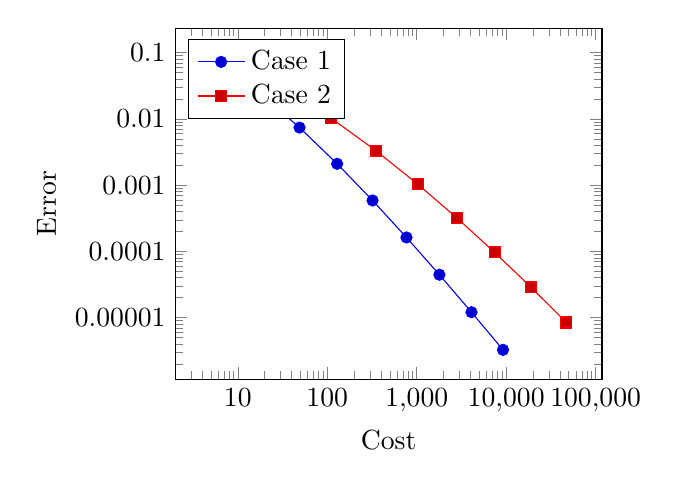
\begin{tikzpicture}
\begin{loglogaxis}[
	log ticks with fixed point,
	xlabel=Cost,ylabel=Error]
\addplot coordinates {
	(5,     8.31160034e-02)
	(17,    2.54685628e-02)
	(49,    7.40715288e-03)
	(129,   2.10192154e-03)
	(321,   5.87352989e-04)
	(769,   1.62269942e-04)
	(1793,  4.44248889e-05)
	(4097,  1.20714122e-05)
	(9217,  3.26101452e-06)
};
\addplot coordinates {
	(7,     8.47178381e-02)
	(31,    3.04409349e-02)
	(111,   1.02214539e-02)
	(351,   3.30346265e-03)
	(1023,  1.03886535e-03)
	(2815,  3.19646457e-04)
	(7423,  9.65789766e-05)
	(18943, 2.87339125e-05)
	(47103, 8.43749881e-06)
};
\legend{Case 1,Case 2}
\end{loglogaxis}
\end{tikzpicture}
\end{codeexample}

	The style replaces |log number format basis|.
\end{stylekey}

\begin{pgfplotskey}{log plot exponent style=\marg{key-value-list}}
Allows to configure the number format of log plot exponents. This style is installed just before `|log number format basis|' will be invoked. Please note that this style will be installed within the default code for `|log number format code|'.
\begin{codeexample}[]
\pgfplotsset{
	samples=15,
	width=7cm,
	xlabel=$x$,
	ylabel=$f(x)$,
	extra y ticks={45},
	legend style={at={(0.03,0.97)},
		anchor=north west}}

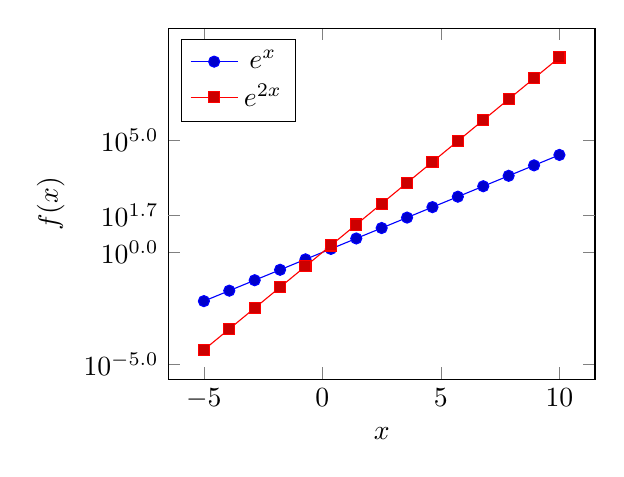
\begin{tikzpicture}
\begin{semilogyaxis}[
	log plot exponent style/.style={
		/pgf/number format/fixed zerofill,
		/pgf/number format/precision=1},
	domain=-5:10]

	\addplot {exp(x)};
	\addplot {exp(2*x)};

	\legend{$e^x$,$e^{2x}$}
\end{semilogyaxis}
\end{tikzpicture}
\end{codeexample}

\begin{codeexample}[]
\pgfplotsset{
	samples=15,
	width=7cm,
	xlabel=$x$,
	ylabel=$f(x)$,
	extra y ticks={45},
	legend style={at={(0.03,0.97)},
		anchor=north west}}

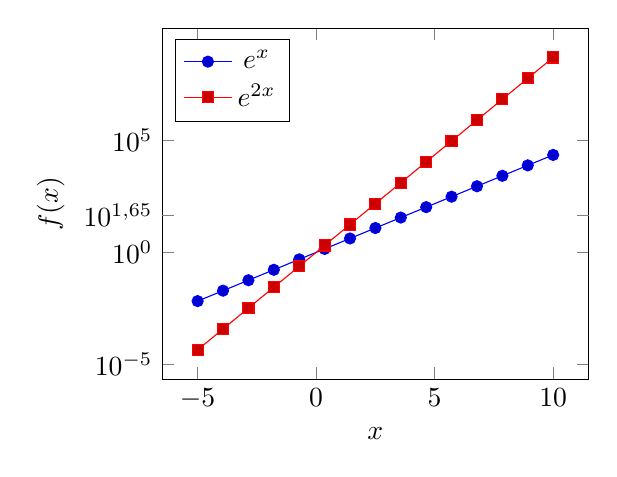
\begin{tikzpicture}
\begin{semilogyaxis}[
	log plot exponent style/.style={
		/pgf/number format/fixed,
		/pgf/number format/use comma,
		/pgf/number format/precision=2},
	domain=-5:10]

	\addplot {exp(x)};
	\addplot {exp(2*x)};

	\legend{$e^x$,$e^{2x}$}
\end{semilogyaxis}
\end{tikzpicture}
\end{codeexample}
\end{pgfplotskey}

\label{sec:identify:minor:log}%
\begin{pgfplotskey}{log identify minor tick positions=\mchoice{true,false} (initially false)}
Set this to |true| if you want to identify log--plot tick labels at positions 
\[ i \cdot 10^j \]
with $i \in \{2,3,4,5,6,7,8,9\},\, j \in \Z$. This may be valuable in conjunction with the `|extra x ticks|' and `|extra y ticks|' options.
\begin{codeexample}[]
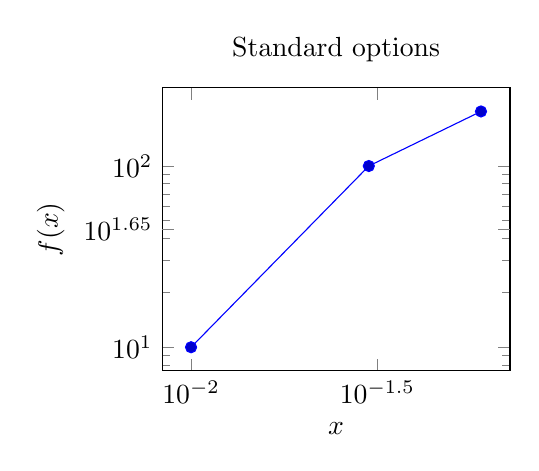
\begin{tikzpicture}%
\begin{loglogaxis}
	[title=Standard options,
	width=6cm]
\addplot coordinates {
	(1e-2,10)
	(3e-2,100)
	(6e-2,200)
};
\end{loglogaxis}
\end{tikzpicture}%
\end{codeexample}

\begin{codeexample}[]
\pgfplotsset{every axis/.append style={%
	width=6cm,
	xmin=7e-3,xmax=7e-2,
	extra x ticks={3e-2,6e-2},
	extra x tick style={major tick length=0pt,font=\footnotesize}
}}%

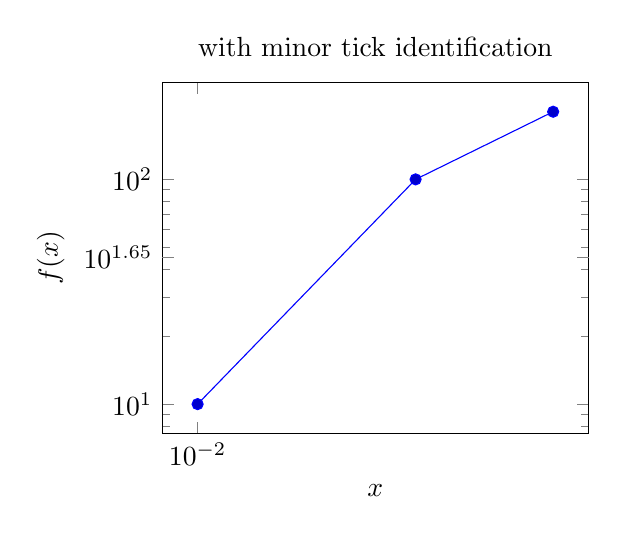
\begin{tikzpicture}%
	\begin{loglogaxis}[
		xtick={1e-2},
		title=with minor tick identification,
		extra x tick style={
			log identify minor tick positions=true}]
	\addplot coordinates {
		(1e-2,10)
		(3e-2,100)
		(6e-2,200)
	};
	\end{loglogaxis}
\end{tikzpicture}%

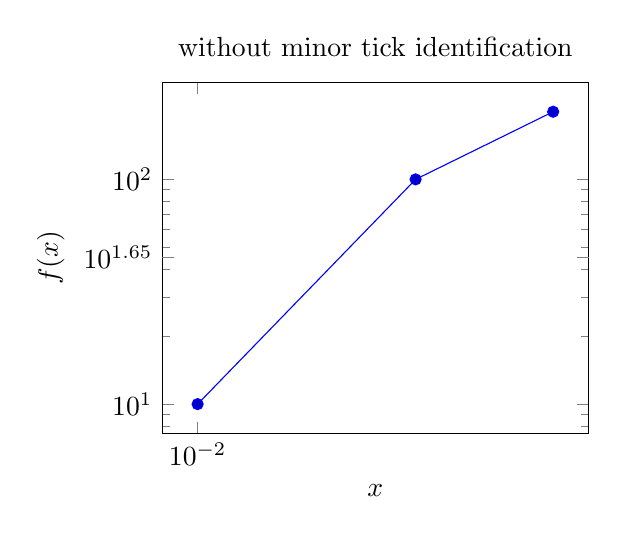
\begin{tikzpicture}%
	\begin{loglogaxis}[
		xtick={1e-2},
		title=without minor tick identification,
		extra x tick style={
			log identify minor tick positions=false}]
	\addplot coordinates {
		(1e-2,10)
		(3e-2,100)
		(6e-2,200)
	};
	\end{loglogaxis}%
\end{tikzpicture}%
\end{codeexample}
	This key is set by the default styles for extra ticks.
\end{pgfplotskey}

\begin{pgfplotscodekey}{log number format code}
Provides \TeX-code to generate log plot tick labels. Argument `|#1|' is the (natural) logarithm of the tick position.
The default implementation invokes |log base 10 number format code| after it changed the log basis to~$10$. It also checks the other log plot options.

This key will have a different meaning when the log basis has been chosen explicitly, see the |log basis x| key.
\end{pgfplotscodekey}


\begin{pgfplotscodekey}{log base 10 number format code}
Allows to change the overall appearance of base 10 log plot tick labels. The default implementation invokes |log number format basis={10}{#1}|.
	
	Use |log plot exponent style| if you only want to change number formatting options for the exponent.
\end{pgfplotscodekey}

\begin{pgfplotscodekey}{log number format basis}
	Typesets a logarithmic tick. The first supplied argument is the log basis, the second the exponent. The initial configuration is
\begin{codeexample}[code only]
\pgfplotsset{
	/pgfplots/log number format basis/.code 2 args={$#1^{\pgfmathprintnumber{#2}}$}
}
\end{codeexample}
	
	Use |log plot exponent style| if you only want to change number formatting options for the exponent.
\end{pgfplotscodekey}


